\documentclass[dvipdfmx]{jsarticle}
\usepackage{amsmath,amssymb}
\usepackage[dvipdfmx]{graphicx}
\usepackage{siunitx}
\usepackage{float}
\usepackage{tikz}
\usepackage{circuitikz}
\usepackage{threeparttable}
\graphicspath{{./figure/}}

\begin{document}
\section{目的}

我々が日常的に電力として利用している電気の多くは交流である。
また回路理論を学ぶ上で、交流及び交流回路の基本的な性質の理解は必要不可欠である。
本実験では、以下の3点を理解することを目的とする。

\begin{itemize}
\item
  交流電圧と周波数の測定方法
\item
  交流電圧波形の解析による交流の諸性質
\item
  交流回路における受動素子の構造と働き
\end{itemize}

\section{原理}

\subsection{正弦波交流の表式}

正弦波交流電圧\(v\)や電流\(i\)は次のような数式で表される。

\begin{eqnarray}
v = V_m\sin(\omega t + \theta_v)\\
i = I_m\sin(\omega t + \theta_i)
\end{eqnarray}

ここでは、\(V_m\)は電圧の最大値、\(\theta_v\)は電圧の位相角、\(\theta_i\)は電流の
位相角、\(t\)は時間\(\omega\)は角周波数を表す。
また、角周波数\(\omega\)と周期\(T\)、周波数\(f\)の関係は次のような式で表される。

\begin{equation}
\omega = \frac{2}{\pi} = 2\pi f[\rm rad/s]
\end{equation}

\subsubsection{瞬時値と実効値}

ある時刻の交流の大きさを瞬時値と言う。実効値は、瞬時値の2乗を1周期の間平均した
値の平方根として定義され、交流の大きさを表すときに使われる。
実効値の物理的な意味は、「交流電圧(電流)を抵抗に加えたときに消費する電力が、
その実効値と同じ大きさの直流電圧(電流)を加えたときの消費電力と等しくなる。」
ということである。 実効値は次の式で求められる。

\begin{eqnarray}
V = \frac{V_m}{\sqrt{2}}, I = \frac{I_m}{\sqrt2}
\end{eqnarray}

\subsection{各種計測器で測定可能な電気的諸量}

本実験で使用する計測器で測定できる電気量を表1に示す。

\begin{table}[h]
  \caption{各種計測器で測定可能な電気的諸量}
  \begin{threeparttable}
    \begin{tabular}{|c|c|c|c|c|c|}\hline 
      \multicolumn{2}{|c|}{電気量} & アナログ回路計 & ディジタルマルチメータ & 交流電子電圧計 & オシロスコープ \\ \hline
      \multicolumn{2}{|c|}{抵抗} & ○\footnotemark[2] & ◎\footnotemark[1] & ×\footnotemark[4] & × \\ \cline{1-6}
      直流 & 電圧 & ○ & ◎ & × & △\footnotemark[3]\\ \cline{2-6}
       & 電流 & ○ & ◎ & × & ×\\ \hline
      交流 & 電圧 & ○ & ○ & ◎ & △\\ \cline{2-6}
       & 電流 & ○ & ○ & × & ×\\ \hline
      \multicolumn{2}{|c|}{周波数} & × & ◎ & × & △\\ \hline
      \multicolumn{2}{|c|}{波形} & ×  & ×  & ×  & ◎ \\ \hline 
    \end{tabular}
    \begin{tablenotes}\footnotesize
      \item[1] 優
      \item[2] 良
      \item[3] 可
      \item[4] 不可
      \end{tablenotes}
\end{threeparttable}
\end{table}
\subsection{リサジュー図形を用いた位相差の測定}

リサジュー図形とは互いに直行する単振動が平面上に描く軌跡である。互いに直行する単振動を

\begin{eqnarray}
  x(t) = A_1\sin(\omega_1 t + \theta_1) \\
	y(t) = A_2\sin(\omega_2 t + \theta_2) 
\end{eqnarray}

とする時、点$(x(t), y(t))を様々なtの値に対して、X-Y平面上$
でプロットして得られる図形がリサジュー図形である。

$x(t)とy(t)$の周波数が等しい場合、リサジュー図形を用いて位相差を求めることができる。

\begin{eqnarray}
  |\sin(\theta_1 - \theta_2)| = \sin^{-1} \frac{b}{a}
\end{eqnarray}

$a$は$x軸方向$の最大値と最小値の差、$b$は$y(t) = 0$を満たす2点の距離である。

\subsection{円筒形コイルのインダクタンスと測定方法}
絶縁された電線を円筒形に一重に巻くことによって作られたコイルのインダクタンス$L$は
次式で与えられる。

\begin{eqnarray}
  L = K \frac{\pi^2 D^2 N^2}{l} \times 10^{-7}
\end{eqnarray}

$Dは直径、lは長さ、Nは巻き数、Kは長岡係数である。$長岡係数とは、直径と長さの比$D/l$で決まる
定数である。

\begin{figure}[h]
  \centering
  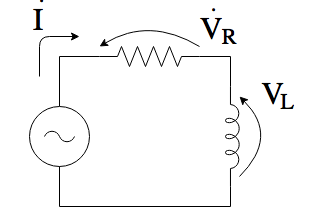
\includegraphics[scale=0.4]{RL_Series_Circut.png}
  \caption{RL直列回路}
  \label{fig:RL_Series_Circuit}
\end{figure}

図\ref{fig:RL_Series_Circuit}に示す
RL直列回路において電圧$\dot V_R, \dot V_L$の実効値(または最大値)と角周波数$\omega、抵抗R$
からインダクタンス$L$を以下の式から求める事ができる。

\begin{eqnarray}
  L = \frac{R}{\omega}\frac{|\dot V_R|}{|\dot V_L|}
\end{eqnarray}

\subsection{平行平板コンデンサのキャパシタンスと測定方法}
同じ形の2枚の金属板を平行に配置する事によって作られた平行平板コンデンサのキャパシタンス
$C$は次式で与えられる。

\begin{eqnarray}
  C = \epsilon_0 \epsilon_r \frac{S}{d}
\end{eqnarray}

$\epsilon_0は真空中の誘電率、\epsilon_rは金属板間を満たす物質の比誘電率、Sは金属板の
面積、dは金属板間の距離である。$

\begin{figure}[h]
  \centering
  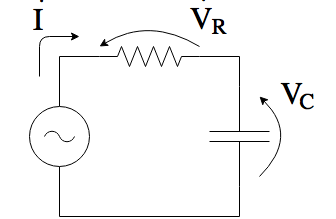
\includegraphics[scale=0.4]{RC_Series_Circuit.png}
  \caption{RC直列回路}
  \label{fig:RC_Series_Circuit}
\end{figure}

図\ref{fig:RC_Series_Circuit}に示すRC直列回路において、電圧$\dot V_R, \dot V_C$の実効値(または最大値)と角周波数$\omega、抵抗R$
から、キャパシタンス$C$を以下の式から求めることができる。

\begin{eqnarray}
  C = \frac{1}{\omega R} \frac{|\dot V_R|}{|\dot V_C|}
\end{eqnarray}
\end{document}